\Chapter{Validáció}

\section{Adathalmaz}

A kínai karaktereket különböző kategóriákba is besorolhatjuk az előállításuk szerint.
\begin{itemize}
\item Nyomtatott: A kijelzőkön megjelenített karakterek. Szélességét és magasságát pixelben adjuk meg. A felbontás növelése minőség növekedést eredményez, de a felismerés ideje nő. Több mint 100 betűtípus létezik.
\item Kézzel írt: A betűtípus íronként változó. Léteznek nagy adathalmazok, ami segíti a gépi tanulást a kínai karakter felismerés során.
\item Generált: Ebben az esetben egy modellt kell létrehozni, ami szerint generálunk. Az alapvonások elhelyezkedésének szabályait figyelembe véve lehetőségünk van bizonyos karakterek generálására.

Grafika szempontjából két csoportra gondolhatunk generálás során.
	\begin{itemize}
	\item Raszteres: Minden egyes képkockának megvan a maga színértéke, így áll össze a kép. Ebben az esetben a számítás igény magas (sok képkocka -> sok számítás).
	\item Vektoros: Gyakorlatilag matematikai képletekkel rajzolunk. Egy egyenes (vektor) pontos meghatározásához három adat szükséges: kiindulópont, végpont koordinátái és a vonalvastagság.
	\end{itemize}
\end{itemize}

A generált adathalmazokat használata elönyös, hiszen nincs hozzáférési kötöttség az adatokhoz. Továbbá rugalmas, hiszen a modell változtatásával könnyedén lehet különböző karaktereket létrehozni (akár nem látottakat is). A minták generálása során vektoros grafikát használtam.

Az adatkészletek gray-scaled képek, 255 pixel értékű háttérképen.

\subsection{A mintaadatok előkészítése a tanításhoz}

A tanító mintáknak különböznie kell a tesztelési mintáktól. A tanítási mintahalmazra a hálózat pontossága magasabb, hiszen a tesztelési pontokat nem ismeri.

Az arányok megválasztásánál gyakori a 80/20 (tanító/tesztelő) arány. Az én esetemben 4GB tanító 1GB tesztelő adathalmazt használok.

Az offline adatokkal végzem el a tanítást.\Aref{fig:offline_dataset}. ábrán láthatunk példát a kínai karakterekre.

\begin{figure}[h]
	\centering
	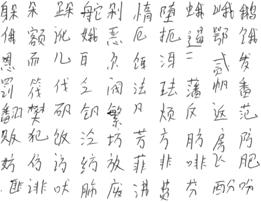
\includegraphics[scale=2.0]{images/offline_dataset}
	\caption{Offline adatbázis példa}
	\label{fig:offline_dataset}
\end{figure} 

Az adathalmaz bejárása előtt azokat érdemes össze keverni véletlenszerűen. Ennek eredménye, hogy a hálózat minden egyes futtatás során egy picivel máshogy fog tanulni. A különbözöségek elkerülésére lehet használni egy úgynevezett \textit{seed}-et, aminek rögzítésekor megegyező módon keveri össze az adatokat. Ehhez a Python \texttt{random} modulja egyszerű megoldást biztosít.
\begin{python}
random.shuffle(self.image_names)
\end{python}

A keverés mellet véletlenszerű zajokat is hozzáadhatunk a képekhez (vágás, forgatás, elmosás). A zaj hozzáadáshoz a \texttt{imgaug} csomag rendkivül hasznos.

\begin{python}
from imgaug import augmenters as iaa

seq = iaa.Sequential([
    iaa.Crop(px=(0, 16)), # vágás 
    iaa.Fliplr(0.5), # horizontális forgatás (50%-ba) 
    iaa.GaussianBlur(sigma=(0, 3.0)) # elmosás 0-3.0 szigma-val
])
\end{python}

A \texttt{imgaug} dokumentációjában részletesen ismertetésre kerülnek az argumentumok (Flipud, Affine, SimplexNoiseAlpha, Dropout, Grayscale, Scale).

\section{A neurális háló tanítása}

\subsection{Mintaadatok beolvasása}

A tanítás elött be kell olvasni a kínai karaktereinket. Mind a tanító mind a tesztelő adathalmaznak ki kell nyerni a címkéjét, ami meghatároza, hogy a kép milyen karakter.

A különböző zajokkal ellátott képeket külön-külön be lehet tanítani a hálózattal. Ebben az esetben szét kell választani a képeket zajok szerint, majd azokat betanítani.

\subsection{Tanítás}

A kép jellemzők kiválasztásához a 4. fejezetben említett konvolúciós hálózatot használom. A CNN a jelenlegi legjobb modellek az objektumok felismerésére, a pontossága 94+\%.

\Aref{fig:arch}. ábra a hálózat architektúrát szemlélteti:

\begin{figure}[h]
	\centering
	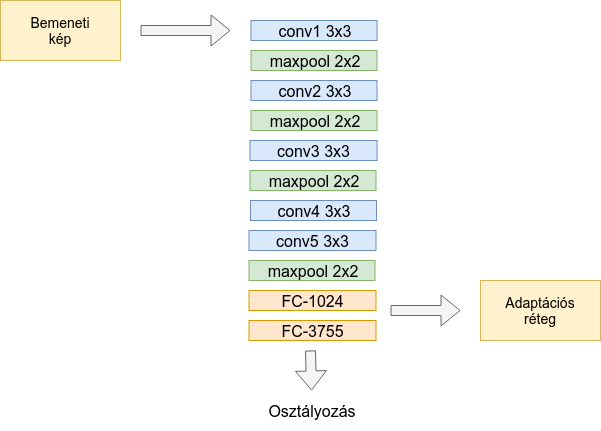
\includegraphics[scale=0.45]{images/architecture}
	\caption{Architektúra}
	\label{fig:arch}
\end{figure}

Ez az alábbi részekből épül fel.
\begin{itemize}
\item Öt konvolúciós (convolution) réteg. Az első réteg megkapja a képet. A kép 64x64 pixel méretű és 1 szín csatorna (gray-scaled) van. A rétegeken 3x3 szűröt (kernel) használok 1-es lépéssel (stride).
\begin{python}
model.add(Convolution2D(1,	# filter rétegek száma    
                        3, 3,	# 3x3 kernel méret 
                        strides=(1,1) # lépés
                        input_shape=image))
\end{python}
\item Négy összevonó (pooling) réteg. Bemenetei a konvolúciós rétegek kimenetei. A rétegen maximális összevonás (max-pooling) van.
\begin{python}
model.add(MaxPooling2D(pool_size=(2,2)))
\end{python}
\item Két teljesen összekötött (fully-connected) réteg. Az aktivációs függvény: RELU, a dropout: 0.2, neuronok száma: 1024, 3755.
\begin{python}
model.add(Flatten()) # Bemenet
model.add(Dense(1024, activation='RELU'))
model.add(Dropout(0.2))
model.add(Dense(3755, activation='None'))
\end{python}
\end{itemize}

A tanítás a 4. fejezetben említett hiba visszaterjesztéssel (backpropagation) történik. A célunk az hogy a hibát megprobáljuk a minimumra csökkenteni, amit a hálózat súlyainak változtatásával érünk el.

\begin{python}
# Negyzetes hiba
model.compile(loss='mean_squared_error',
              optimizer='adam',
              metrics=['accuracy'])

# Halozat tanitas
model.fit_generator(generator=training_data,
                    steps_per_epoch=1000, epochs=10)
\end{python}

A tanítás ideje körülbelül 17 órát vett igénybe. A hardver: CPU - 4 mag 2.8Ghz, RAM - 4Gb. Tanítási lépések 3200epoch, tanítóhalmaz méret: 300Mb.

\section{Tesztelés}

A tesztelés során megvizsgálom, hogy mennyire érzékenyek az adott zajok a hálózatra. A tanítás fázisnál figyelembe kell venni kell venni azt, hogy ha ugyanolyan zajjal tanítjuk be a  hálózatot akkor azt csak azt fogja jól felismerni. Előállhat az overfitting.

Felismerés zajok szerint:
\begin{itemize}
\item Zaj nélküli: A kép zajjal nincs terhelve. A felismerés ebben az esetben a legmagasabb a zaj nélküli mintákra (90+\%), viszont a zajosított képeket nehezen ismeri fel.\Aref{fig:original} ábrán látható az eredti kép.

\begin{figure}[h]
	\centering
	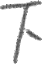
\includegraphics[scale=1.0]{images/original}
	\caption{Eredeti kép}
	\label{fig:original}
\end{figure}

\item Pontszerű: A tanítást pontszerű zajjal terhelt képekre végezzük el. A rendszer nehezebben ismeri fel az utóbbi mintákat (75-80\%) és a zajnélküli mintákat (90+->84\%) is. A pontszerű zajok nem okoznak nagy problémát, hiszen a konvolúciós réteg az összevonó réteg megfelelő paraméterizálása megoldja a gondot.\Aref{fig:noise} ábrán látható a zajosított kép.

\begin{figure}[h]
	\centering
	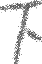
\includegraphics[scale=1.0]{images/noise}
	\caption{Pontszerű zaj}
	\label{fig:noise}
\end{figure}

\item Forgatás A tanítás elforgatott képekkel. A $\pm$5-20 fokos origó körüli forgatás kis mértékben változtatja meg a hálózat felismerését. A nagyobb forgatások nagyon megnehezítik a képek felismerését (zaj nélküli: 92\%->78\%, pontszerű: 80\%->70\%). Azzal magyarázható hogy a forgatás során az alapvonások helyzete, iránya, vektorai megváltoznak. \Aref{fig:rotated} ábrán látható az elforgatott kép.

\begin{figure}[h]
	\centering
	
\includegraphics[scale=1.0]{images/rotate}
	\caption{Elforgatott kép}
	\label{fig:rotated}
\end{figure}
\newpage
\item Elmosás: A tanítás homályos/elmosódott képekkel. Kis mértékben befolyásolja a hálózat felismerés aranyát. A hálózat jól alkalmazkodik a homályosított képhez.\Aref{fig:blur} ábrán látható az elmosódott kép.

\begin{figure}[h]
	\centering
	
\includegraphics[scale=1.0]{images/blur}
	\caption{Elmosódott kép}
	\label{fig:blur}
\end{figure}

\end{itemize}